\def\inc{inc1-3-dev}

\titreA {Gestion des périphériques}

%%%%%%%%%%%%%%%%%%%%%%%%%%%%%%%%%%%%%%%%%%%%%%%%%%%%%%%%%%%%%%%%%%%%%%%%%%%%%%
% Introduction
%%%%%%%%%%%%%%%%%%%%%%%%%%%%%%%%%%%%%%%%%%%%%%%%%%%%%%%%%%%%%%%%%%%%%%%%%%%%%%

\titreB {Introduction}

\begin {frame} {Introduction}
    \begin {center}
	\includegraphics [width=.7\linewidth] {\inc/arch-old}
    \end {center}

    Sous Unix, les périphériques sont accédés comme des fichiers
    \\
    \implique adage « tout est fichier »
\end {frame}

\begin {frame} {Introduction}
    \begin {itemize}
	\item imprimer sur l'imprimante~:
	    \lstinputlisting [basicstyle=\fD\lstmonstyle] {\inc/lpr.c}
	\item lire le contenu d'un disque dur :
	    \lstinputlisting [basicstyle=\fD\lstmonstyle] {\inc/dsk.c}
    \end {itemize}

    Où est la magie ?
\end {frame}

\begin {frame} {Nouveaux types de fichiers}
    Deux nouveaux types de fichiers spéciaux (périphériques) :
    \ctableau {\fD} {|p{.45\linewidth}|p{.45\linewidth}|} {
	\rc \multicolumn {1} {|c|} {\textbf {mode « caractère »}}
	    & \multicolumn {1} {c|} {\textbf {mode « bloc »}}
	    \\ \hline
	\rc avec \code {stat} : \code {S\_IFCHR} et \code {S\_ISCHR()}
	    & avec \code {stat} : \code {S\_IFBLK} et \code {S\_ISBLK()}
	    \\
	\rc aurait dû s'appeler : mode « brut »
	    & aurait dû s'appeler : mode « bufferisé »
	    \\
	\rc toute suite d'octets passée à \code {read} ou
		\code {write} est transférée immédiatement
	    & toute suite d'octets passée à \code {read} ou
		    \code {write} est bufferisée, avant d'être
		    transférée sur le périphérique
	    \\
	\rc tous les périphériques ou presque
	    & essentiellement les disques durs
	    \\
	\rc périphérique identifié par un couple
		<\textit {majeur}, \textit {mineur}>
	    & périphérique identifié par un couple
		<\textit {majeur}, \textit {mineur}>
	    \\
    }

    \vspace* {3mm}

    Fichiers localisés (traditionnellement) dans \code {/dev}

\end {frame}

\begin {frame} {Numéro de périphérique}
    Périphériques identifiés par un couple <majeur, mineur>

    \ctableau {\fB} {|l|l|} {
	\rc majeur & numéro de pilote (brut ou bufferisé) \\
	\rc mineur & numéro de périphérique géré par ce pilote \\
	\rc & (+ autres informations éventuellement)
	    \\
    }

    \begin {itemize}
	\item Exemple : pilote de disques « sd » (Linux)
	    \begin {itemize}
		\item majeur = 8
		\item mineur = adresse du disque (bits $\geq$ 4) +
		    numéro de partition (bits 0..3)
	    \end {itemize}
	\item type \code {dev\_t} : majeur + mineur

    \end {itemize}
\end {frame}

\begin {frame} {Fichiers périphériques -- Création}
    \prototype {
	\code {int mknod (const char *path, mode\_t mode, dev\_t dev)}
    }

    \begin {itemize}
	\item crée un fichier périphérique
	\item primitive restreinte à l'administrateur du système
	\item \code {mode} : analogue à \code {st\_mode} (type
	    et permissions)
	\item usage non supporté par POSIX
	\item primitive désuette : périphériques créés automatiquement
    \end {itemize}
\end {frame}

\begin {frame} {Fichiers périphériques -- Primitive stat}
    Retour sur \code {stat} :

    \begin {itemize}
	\item si le fichier est un périphérique (bloc ou caractère)
	    \begin {itemize}
		\item champ \code {st\_mode} testé avec \code {S\_ISBLK()}
		    ou \code {S\_ISCHR()}

		\item champ \code {st\_rdev} : numéro du périphérique
	    \end {itemize}

	\item pour tous les fichiers

	    \begin {itemize}
		\item réguliers, répertoires, liens symboliques,
		    périphériques, etc
		\item le fichier réside sur un disque \item champ \code
		{st\_dev} : numéro de périphérique
		    du disque
	    \end {itemize}
    \end {itemize}
\end {frame}

%%%%%%%%%%%%%%%%%%%%%%%%%%%%%%%%%%%%%%%%%%%%%%%%%%%%%%%%%%%%%%%%%%%%%%%%%%%%%%
% Pilotes de périphériques
%%%%%%%%%%%%%%%%%%%%%%%%%%%%%%%%%%%%%%%%%%%%%%%%%%%%%%%%%%%%%%%%%%%%%%%%%%%%%%

\titreB {Pilotes de périphériques}

\begin {frame} {Pilotes de périphérique}
    \begin {itemize}
	\item pilote de périphérique :
	    \begin {itemize}
		\item ensemble de fonctions
		\item code compilé ajouté au noyau
		\item fonctions référencées dans la table des
		    pilotes du noyau
	    \end {itemize}
	\item fonctions différentes suivant le type de pilote :
	    \ctableau {\fC} {|p{.45\linewidth}|p{.45\linewidth}|} {
		\rc \multicolumn {1} {|c|} {\textbf {mode « caractère »}}
		    & \multicolumn {1} {c|} {\textbf {mode « bloc »}}
		    \\ \hline
		\rc fonctions \code {open}, \code {close}, \code {read},
		    \code {write}, \code {ioctl} et interruption
		    & fonctions \code {open}, \code {close}, \code
		    {strategy} et interruption
		    \\
	    }
    \end {itemize}
\end {frame}

\begin {frame} {Pilotes de périphérique}
    Cheminement d'une requête :

    \begin {center}
	\includegraphics [width=1\linewidth] {\inc/cdevsw}
    \end {center}

\end {frame}

\begin {frame} {Mode caractère}
    Interface du pilote :
    \begin {itemize}
	\item fonctions \code {open}, \code {close}, \code {read} et
	    \code {write} : bien connues
	\item traitement d'interruption : appelée lorsqu'une interruption
	    est générée à la fin du traitement par le périphérique
	\item fonction \code {ioctl} : correspond à la primitive
	    \vspace* {-1mm}
	    \prototype {
		\code {int ioctl (int fd, int requete, .... paramètre)}
	    }
	    \begin {itemize}
		\item non normalisée par POSIX (pour les périphériques)
		\item opérations spécifiques
		    qui ne rentrent pas dans le modèle read/write
		\item exemples :
		    \begin {itemize}
			\item interroger l'imprimante pour connaître 
			    son état (en cours d'impression, plus de
			    papier, etc.)

			\item éjecter le support (cartouche magnétique,
			    CD, DVD, etc.)

			\item changer la vitesse de la liaison série
		    \end {itemize}
	    \end {itemize}
    \end {itemize}
\end {frame}

\begin {frame} {Mode caractère}
    Un exemple particulier : le terminal (télétype)

    \vspace* {3mm}

    \begin {minipage} [c] {.30\linewidth}
	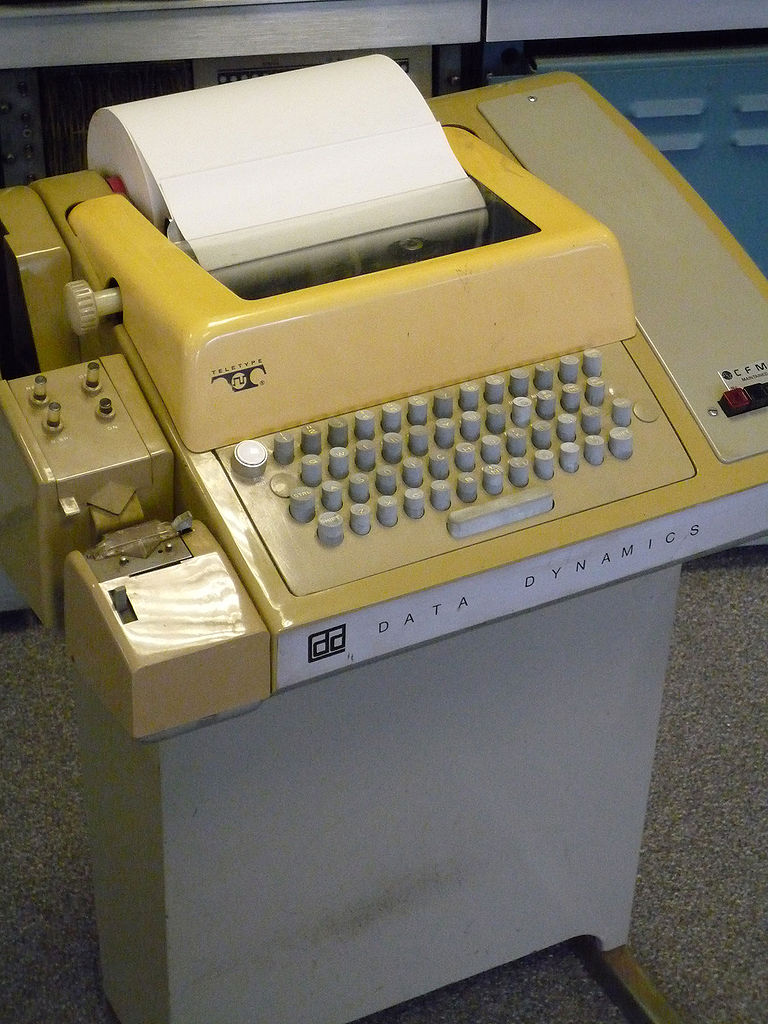
\includegraphics [width=\linewidth] {\inc/tty}
    \end {minipage}
    \hfill
    \begin {minipage} [c] {.68\linewidth}
	\begin {itemize}
	    \fB
	    \item il est relié par un lien série
		\begin {itemize}
		    \fC
		    \item paramètres : vitesse du lien, nombre
			de bits, parité
		    \item raccrocher le modem en fin de connexion
		    \item etc.
		\end {itemize}
	    \item il a des caractéristiques propres
		\begin {itemize}
		    \fC
		    \item caractères d'effacement, d'arrêt, de
			suspension, de fin de fichier, etc
		    \item bufferiser les caractères par ligne ou les
			envoyer sans attendre
		    \item nombre de lignes, de colonnes
		    \item etc.

		\end {itemize}
	\end {itemize}
    \end {minipage}

    \vspace* {2mm}

    \implique commande \code {stty} pour changer les paramètres (\implique
    \code {ioctl})

\end {frame}

\begin {frame} {Mode caractère}
    Un exemple particulier : le terminal (télétype)

    \begin {itemize}
	\fB
	\item le pilote a pour mission d'acheminer les octets
	    jusqu'au terminal

	\item certains programmes (ex: \code {zsh}, \code {vi},
	    \code {more}, etc.) doivent pouvoir en plus effacer l'écran,
	    positionner le curseur à un certain endroit, reconnaître
	    les touches de fonction, etc.

	\item séquences de contrôle différentes suivant les terminaux
	\item positionner le curseur à la ligne X et colonne Y : il faut envoyer...
	    \begin {itemize}
		\fD
		\item \framebox {ESC} \framebox {[} X \framebox {;}
		    Y \framebox {f} pour un terminal DEC VT100

		\item \framebox {ESC} \framebox {\&} \framebox {a}
		    Y \framebox {c} X \framebox {Y} pour un terminal
		    HP 2645

		\item Note : \framebox {ESC} = l'octet de code 27
	    \end {itemize}

	\item base \code {termcap}, puis \code {terminfo} pour l'ensemble
	    des séquences
	    \begin {itemize}
		\item variable d'environnement \code {TERM} : indique
		    le type de terminal
	    \end {itemize}

	\item les programmes (\code {zsh}, \code {vi}, etc.) doivent
	    utiliser cette base
	    \\
	    \implique ce n'est pas la mission du pilote

    \end {itemize}
\end {frame}

\begin {frame} {Mode caractère}
    Même principe pour la plupart des périphériques :

    \begin {itemize}
	\item le pilote achemine les octets jusqu'au périphérique
	\item ceci ne dispense pas les applications de gérer le
	    protocole de chaque périphérique

	    \begin {itemize}
		\item plusieurs protocoles différents pour les souris \\
		    \implique seul le serveur X-Window doit les connaître
		\item chaque imprimante dispose de son « langage de
		    contrôle »
		    \\
		    \implique tout programme souhaitant imprimer doit
		    disposer d'une collection d'adaptateurs pour les
		    différentes imprimantes (parfois nommés à tort
		    « pilotes »)
		\item etc.

	    \end {itemize}
    \end {itemize}
\end {frame}

\begin {frame} {Mode bloc}
    Interface du pilote :
    \begin {itemize}
	\item fonctions \code {open}, \code {close} : appelées au
	    montage/démontage du système de fichiers dans l'arborescence
	\item traitement d'interruption : idem mode brut
	\item fonction \code {strategy} : 2 rôles
	    \begin {itemize}
		\item lit un bloc en mémoire, dans le «~\textit {buffer
		    cache}~» (plus tard)
		\item écrit un bloc modifié du «~\textit {buffer cache}~»
		    vers le disque
		\item permet d'implémenter des optimisations \\
		    (ex : algorithme de l'ascenseur)
	    \end {itemize}
    \end {itemize}

    \vspace* {2mm}

    Note : la plupart des pilotes en mode bloc sont également
    accompagnés d'un pilote en mode caractère (pour \code {ioctl})
\end {frame}

\begin {frame} {Pseudo-périphériques}
    Un pilote peut offrir un service accessible via \code {read}
    ou \code {write} sans qu'il y ait un vrai périphérique

    \vspace* {3mm}

    Exemples :

    \ctableau {\fB} {|l|l|} {
	\rc \code {/dev/null} & poubelle \\
	\rc \code {/dev/mem} & toute la mémoire de l'ordinateur \\
	\rc \code {/dev/random} & source d'aléa \\
    }

\end {frame}

\begin {frame} {Pseudo-périphériques}
    Cas particulier : les pseudo-terminaux

    \begin {itemize}
	\item beaucoup de programmes sont conçus pour être connectés
	    à un terminal

	\item comment fait \code {vi} lorsqu'on est connecté via
	    \code {ssh} ou via un terminal X-Window ?
	    \\
	    \implique il faut simuler un terminal et un lien série

	\item abstraction : pseudo-terminal

	    \begin {itemize}
		\item paire de pseudo-périphériques : maître et esclave
		\item gérés par le même pilote
		\item le serveur ssh gère le maître
		\item les programmes de la session accèdent
		    à l'esclave : il simule un « vrai » terminal
	    \end {itemize}
    \end {itemize}
\end {frame}

\begin {frame} {Pseudo-périphériques}

    \begin {minipage} [c] {.40\linewidth}
	\includegraphics [width=\linewidth] {\inc/pty}
    \end {minipage}
    \hfill
    \begin {minipage} [c] {.58\linewidth}
	\begin {itemize}
	    \fB
	    \item le serveur ssh ouvre la paire
	    \item tout octet émis vers le maître (resp. esclave)
		est transmis vers l'esclave (resp. maître)
	    \item le serveur ssh transmet les octets reçus depuis
		le réseau vers le maître
	    \item les programmes de la session ssh (\code {sh},
		\code {vi}) sont connectés à l'esclave
	    \item tout changement de paramètre terminal (via \code {ioctl})
		est transmis au serveur ssh
	\end {itemize}
    \end {minipage}

    \begin {itemize}
	\item autres utilisations :
	    \begin {itemize}
		\item fenêtres « terminal » en environnement graphique
		\item \code {script} (enregistrement de session)
		\item programmes \code {screen} et \code {tmux}
	    \end {itemize}
    \end {itemize}

\end {frame}

\begin {frame} {Évolutions}
    Réalité : malheureusement très complexe...
    \begin {center}
	\includegraphics [width=.6\linewidth] {\inc/arch-now}
    \end {center}

    Exemple : disques connectés via le bus SATA, SCSI,
    USB ou même via un ancestral bus IDE.

\end {frame}

\begin {frame} {Évolutions}
    \begin {itemize}
	\item complexité matérielle accrue

	    \begin {itemize}
		\item gestion des différents niveaux de bus
		\item partage de code entre pilotes (exemple : disques)
	    \end {itemize}

	\item dynamicité des périphériques

	    \begin {itemize}
		\item connecter ou déconnecter des périphériques « à chaud »
		\item auto-reconnaissance des périphériques
	    \end {itemize}
    \end {itemize}

    \implique complexité des pilotes
\end {frame}


%%%%%%%%%%%%%%%%%%%%%%%%%%%%%%%%%%%%%%%%%%%%%%%%%%%%%%%%%%%%%%%%%%%%%%%%%%%%%%
% Le répertoire /dev
%%%%%%%%%%%%%%%%%%%%%%%%%%%%%%%%%%%%%%%%%%%%%%%%%%%%%%%%%%%%%%%%%%%%%%%%%%%%%%

\titreB {Le répertoire /dev}

\begin {frame} {Le répertoire /dev}
    Historiquement, le répertoire \code {/dev} était peuplé «~à
    la main~»

    \begin {itemize}
	\item peu d'ajout ou de suppression de périphériques
	\item commande \code {mknod}
	\item script \code {MAKEDEV} dans \code {/dev}
    \end {itemize}
\end {frame}

\begin {frame} {Le répertoire /dev}
    Évolution \implique ajout dynamique de périphériques

    \begin {itemize}

	\item Système de fichier « devfs »

	    \begin {itemize}
		\item création/destruction automatique des fichiers spéciaux
		\item nécessite des périphériques capables de s'identifier
		    \begin {itemize}
			\item « plug and play »
		    \end {itemize}
	    \end {itemize}

	\item Programme additionnel pour gérer les exceptions

	    \begin {itemize}
		\item je veux un lien \code {/dev/cédérom} vers le
		    troisième lecteur de CD de mon système

		\item je veux pouvoir connecter mon appareil photo
		    sans avoir les droits de l'administrateur
	    \end {itemize}
    \end {itemize}
\end {frame}
